\subsection{Compression of a plate with a hole}
\label{subsec:Mp1}

\subsubsection{Definition}
\label{subsubsec:Mp1_def}

Compression and/or tension of a plate with a hole is a typical plane strain benchmark for the modeling of elastoplastic material behavior, and is defined in \cite{SteEtAl:03}. Here, this example is analyzed to compare the behavior of two approaches on pure plastic deformation problems. 

\subsubsection{Solution}
\label{subsubsec:Mp1_sol}

In the present simulation, a quarter of the perforated plate is considered because of the symmetry of the problem. The model set-up is shown in Fig.~\ref{Mp_ex1_model}. The radius of the hole is $10\,$mm. Two points (point~1 and point~2) are specified to monitor the evolution of variables. Point~1 is located at one third of the distance from point~3 to point~4.

\begin{figure}[!htb]
\centering
    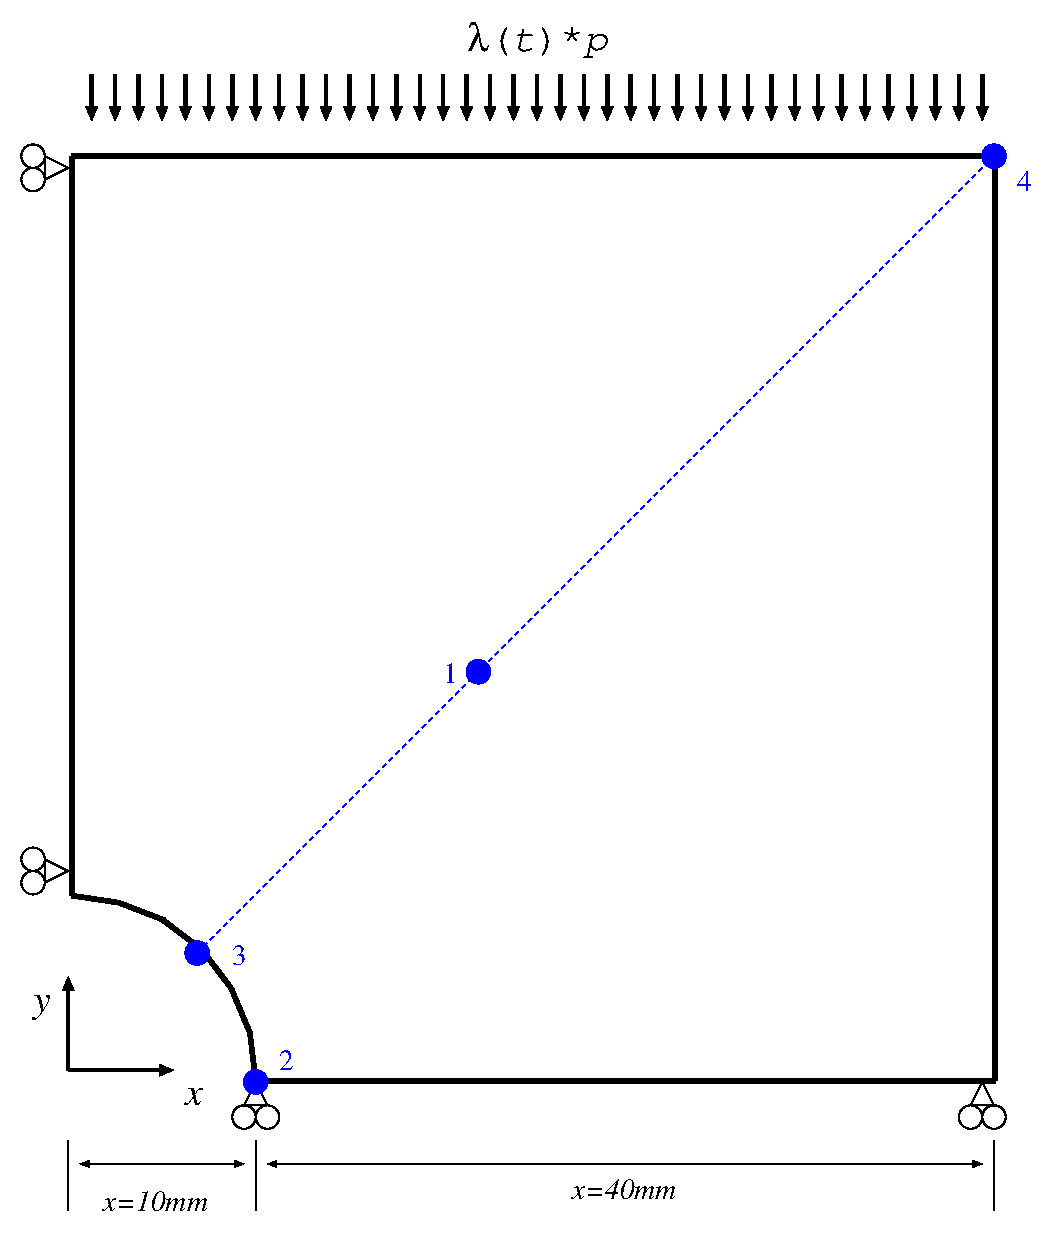
\includegraphics[scale=0.3]{PART_II/M/ex1_model.eps}\\
   \caption{One quarter of the compressed steel plate with a hole}
  \label{Mp_ex1_model}
\end{figure}

Traction boundary conditions, $p=100\cdot\lambda(t)\,$MPa are prescribed on the top,  where $\lambda(t)$ denotes a time-dependent scaling factor. The particular case of cycling loading is analyzed defining a scaling factor as shown in Fig.~\ref{Mp_ex1_load} assuming $\lambda_{\mathrm{max}}=4.1$.

The finite element grid using triangular elements is shown in Fig.~\ref{Mp_ex1_mesh}, and the material parameters obtained from \cite{SteEtAl:03} are presented in Table~\ref{Mp_ex1_table1}.

\begin{figure}[!thb]
\centering
    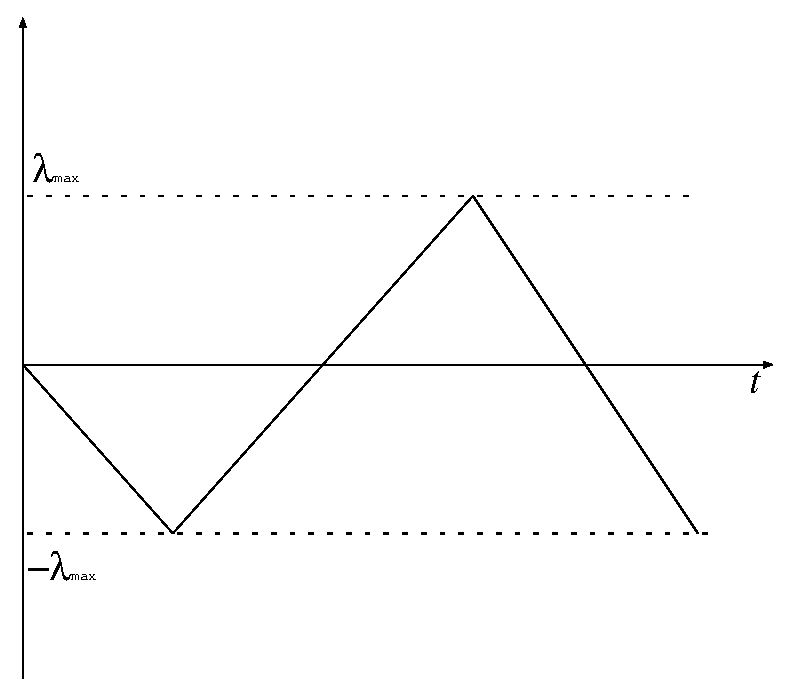
\includegraphics[scale=0.5]{PART_II/M/ex1_load.eps}\\
   \caption{Time dependent scaling factor for external loading}
  \label{Mp_ex1_load}
\end{figure}

\begin{figure}[!htb]
\centering
    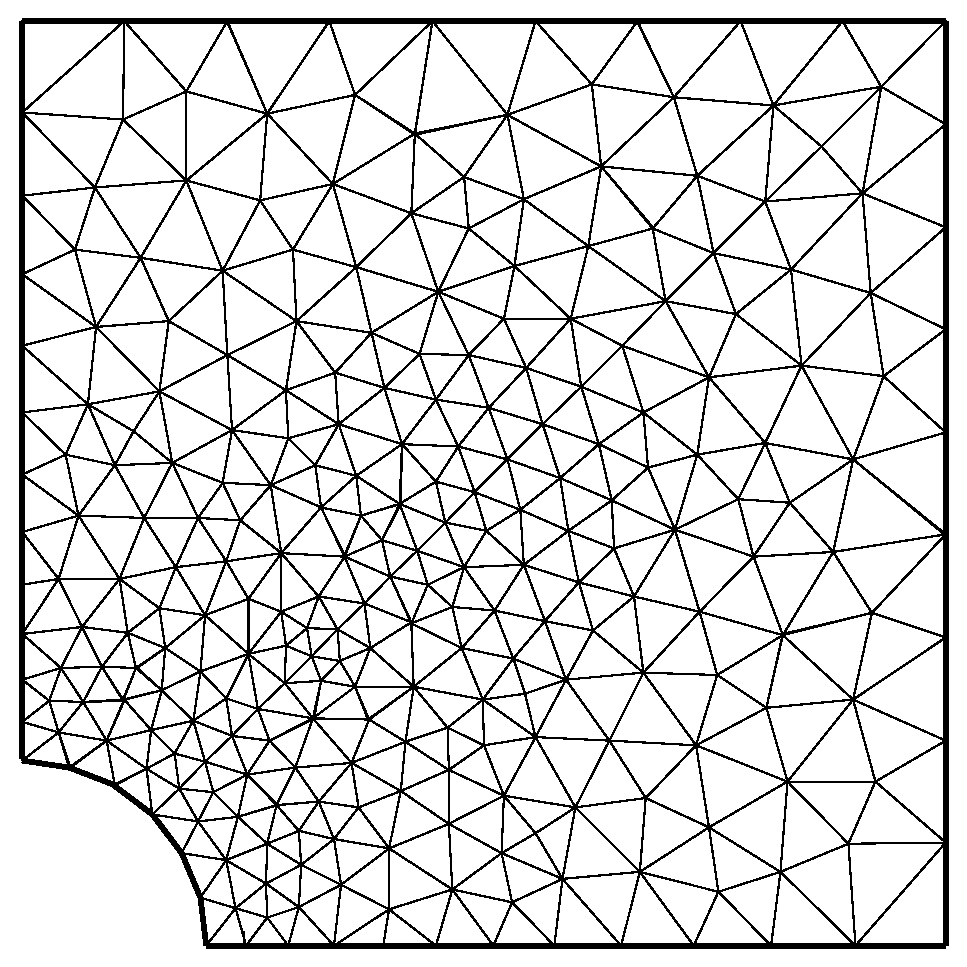
\includegraphics[scale=0.3]{PART_II/M/ex1_mesh_gfem.eps}\\
   \caption{Finite element grid: 269 nodes and 484 elements}
  \label{Mp_ex1_mesh}
\end{figure}

\begin{table}[!htb]
\centering
\caption{Material parameters}
\label{Mp_ex1_table1}
\begin{tabular}{llll}
\toprule
Symbol & Parameter & Value & Unit \\
\midrule
$E$        & Young's modulus      & $206.9$ & GPa \\
$\nu$      & Poisson's ratio      & $0.29$  & --  \\
$\sigma_0$ & Initial yield stress & $0.45$  & GPa \\
\bottomrule
\end{tabular}
\end{table}

\subsubsection{Results}
\label{subsubsec:Mp1_res}

The load is applied within 60 time steps with a constant increment for the loading factor $\Delta\lambda=\lambda_{\mathrm{max}}/10$. As shown in Fig.~\ref{Mp_ex2_cont1}, plastic strain and vertical strain show similar distributions, which are typical for elastoplastic material behavior according to the von~Mises model. The evolution of the horizontal displacement at point~1 and at point~2 as functions of the periodic scaling factor $\lambda (t)$ are shown on Fig.~\ref{Mp_ex2_loadp}.

%Contour plot
\begin{figure}[!thb]
  \begin{center}
   \begin{minipage}[t]{0.48\textwidth}
     \begin{center}
    \includegraphics[scale=0.28]{PART_II/M/ex1_pls_4.1.eps}
    \centerline{(Plastic strain)}
    \end{center}
   \end{minipage}
   \hspace{0.02\textwidth}
   \begin{minipage}[t]{0.48\textwidth}
    \begin{center}
    \includegraphics[scale=0.28]{PART_II/M/ex1_strain_yy_4.1.eps}\\
    \centerline{(Vertical strain)}
    \end{center}
   \end{minipage}\\
   %
  \end{center}
  \caption{Distribution of plastic strain and vertical strain at $\lambda_{\mathrm{max}}/10$}
  \label{Mp_ex2_cont1}
\end{figure}

\begin{figure}[!htb]
  \begin{center}
   \begin{minipage}[t]{0.48\textwidth}
     \begin{center}
    \includegraphics[scale=0.28]{PART_II/M/ex1_load_v_ux_p1.eps}
    \centerline{(Point 1)}
    \end{center}
   \end{minipage}
   \hspace{0.02\textwidth}
   \begin{minipage}[t]{0.48\textwidth}
    \begin{center}
    \includegraphics[scale=0.28]{PART_II/M/ex1_load_v_ux_p2.eps}\\
    \centerline{(Point 2)}
    \end{center}
   \end{minipage}\\
   %
  \end{center}
  \caption{Evolution of horizontal displacement vs. scaling factor}
  \label{Mp_ex2_loadp}
\end{figure}
